\documentclass[twocolumn,superscriptaddress,showpacs,preprintnumbers,amsmath,amssymb,prl]{revtex4-1}
\usepackage{siunitx}
\usepackage{tikz}
\usetikzlibrary{arrows,shapes,backgrounds, calc, positioning, topaths,chains, intersections, decorations.markings, shapes.geometric, matrix,patterns,mindmap,fit}
%\usetikzlibrary{positioning, patterns,topaths,chains,matrix}

\usepackage{pgfplots}
\pgfplotsset{compat=1.9}
\usepgfplotslibrary{groupplots}
\usepgfplotslibrary{external}
\tikzsetexternalprefix{fig_plis/}
\tikzexternalize
\tikzset{external/force remake}



\definecolor{Main}{rgb}{1, 0.57, 0}
\definecolor{Accent1}{rgb}{1,0.28,0}
\definecolor{Accent2}{rgb}{1,0.74,0}

\begin{document}
\author{Mathieu Leocmach}

\begin{figure}
	\tikzsetnextfilename{dynamics}
	% \begin{figure*}
% 	\begin{tikzpicture}
% 	\matrix[matrix of nodes, inner sep=0, column sep=0.015\textwidth, row sep=0.5em] (m){
% 	33 min & 38 min & 43 min & 48 min & 1h & 1h15 & 2h30\\
% 	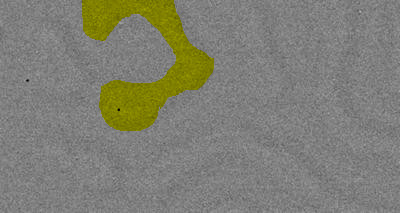
\includegraphics[width=0.13\textwidth]{prise_0100_color.jpg}&
% 	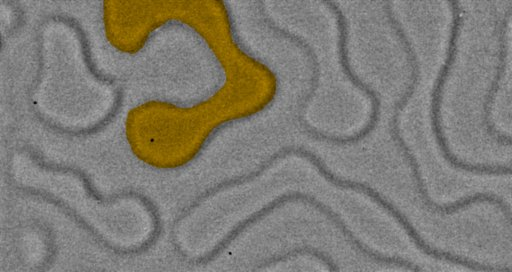
\includegraphics[width=0.13\textwidth]{prise_0130_color.jpg}&
% 	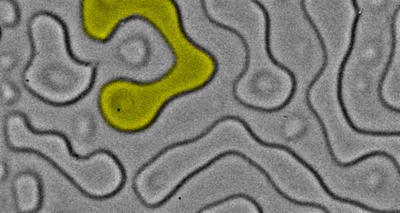
\includegraphics[width=0.13\textwidth]{prise_0160_color.jpg}&
% 	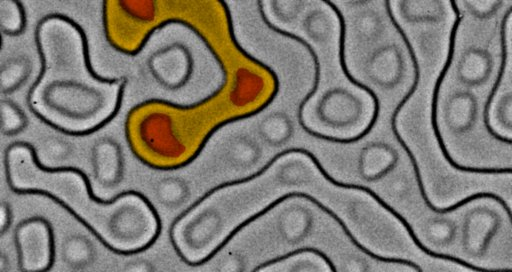
\includegraphics[width=0.13\textwidth]{prise_0190_color.jpg}&
% 	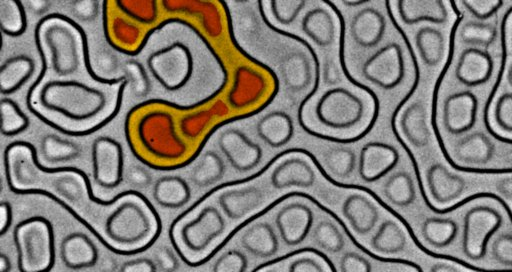
\includegraphics[width=0.13\textwidth]{prise_0250_color.jpg}&
% 	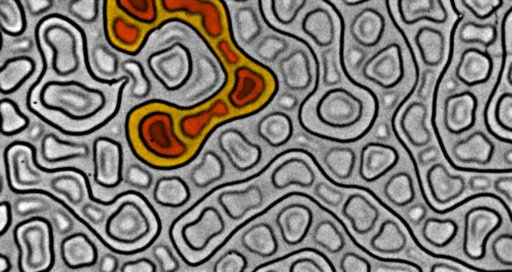
\includegraphics[width=0.13\textwidth]{prise_0360_color.jpg}&
% 	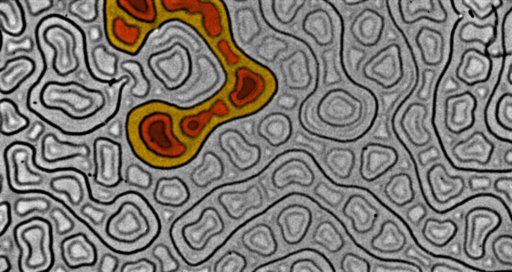
\includegraphics[width=0.13\textwidth]{prise_0799_color.jpg}\\
% 	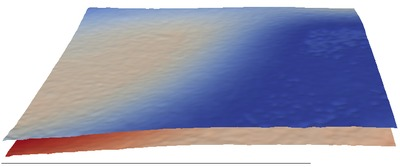
\includegraphics[width=0.13\textwidth]{cas3p2_fluo0p8_GDL4_2_t047_crop_resized.jpg}&
% 	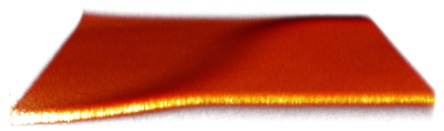
\includegraphics[width=0.13\textwidth]{cas3p2_fluo0p8_GDL4_2_t056_crop_resized.jpg}&
% 	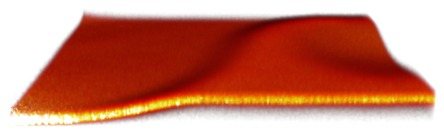
\includegraphics[width=0.13\textwidth]{cas3p2_fluo0p8_GDL4_2_t065_crop_resized.jpg}&
% 	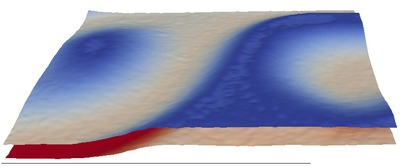
\includegraphics[width=0.13\textwidth]{cas3p2_fluo0p8_GDL4_2_t074_crop_resized.jpg}&
% 	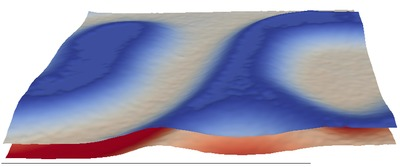
\includegraphics[width=0.13\textwidth]{cas3p2_fluo0p8_GDL4_2_t092_crop_resized.jpg}&
% 	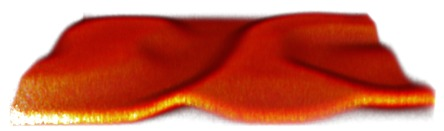
\includegraphics[width=0.13\textwidth]{cas3p2_fluo0p8_GDL4_2_t125_crop_resized.jpg}&
% 	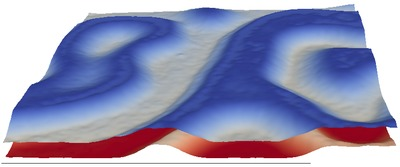
\includegraphics[width=0.13\textwidth]{cas3p2_fluo0p8_GDL4_2_t260_crop_resized.jpg}\\
% 	};
% 	\draw[ultra thick] ++(m-2-1.south west) -- ++(0.023\textwidth,0);
% 	\draw[ultra thick] ++(m-3-1.south west) -- ++(0.1\textwidth,0);
% 	\end{tikzpicture}
% 	\caption{Dynamics of pattern formation for $e\approx\SI{100}{\micro\metre}$. (top) By light transmission microscopy. (bottom) Reconstructed from fluorescent confocal microscopy (corresponds to the squared area in Fig.~\ref{fig:acidgel}e). Scale bars are \SI{1}{\milli\metre}.}
% 	\label{fig:dynamics}
% \end{figure*}
%\begin{figure}
\begin{tikzpicture}
\matrix[matrix of nodes, inner sep=0, column sep=0.0\columnwidth, row sep=0.5em, column 1/.style={base left},nodes={anchor=center},] (m){
	\SI{33}{\minute} & 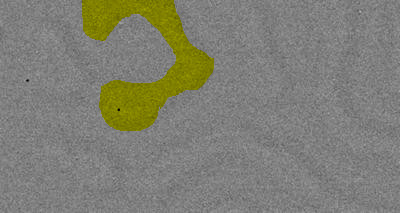
\includegraphics[height=4.5em]{prise_0100_color.jpg}&
	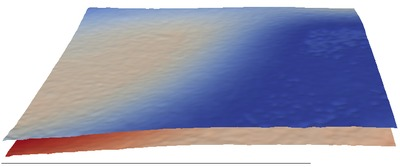
\includegraphics[height=4.5em]{cas3p2_fluo0p8_GDL4_2_t047_crop_resized.jpg}\\
	\SI{38}{\minute} & 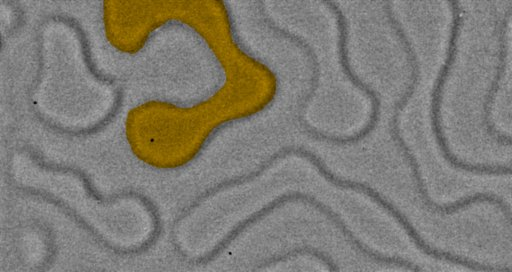
\includegraphics[height=4.5em]{prise_0130_color.jpg}&
	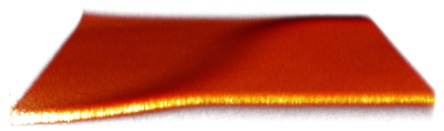
\includegraphics[height=4.5em]{cas3p2_fluo0p8_GDL4_2_t056_crop_resized.jpg}\\
	\SI{43}{\minute} & 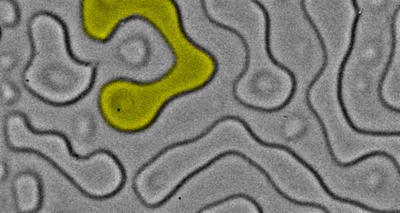
\includegraphics[height=4.5em]{prise_0160_color.jpg}&
	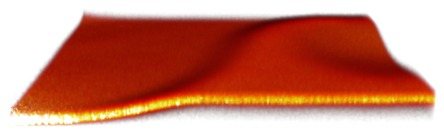
\includegraphics[height=4.5em]{cas3p2_fluo0p8_GDL4_2_t065_crop_resized.jpg}\\
	\SI{48}{\minute} & 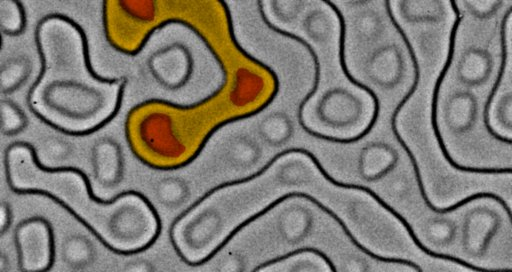
\includegraphics[height=4.5em]{prise_0190_color.jpg}&
	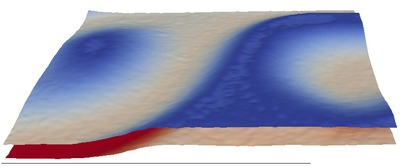
\includegraphics[height=4.5em]{cas3p2_fluo0p8_GDL4_2_t074_crop_resized.jpg}\\
	\SI{1}{\hour} & 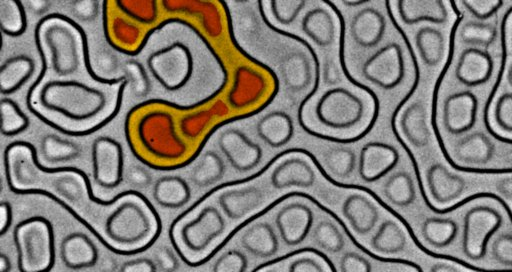
\includegraphics[height=4.5em]{prise_0250_color.jpg}&
	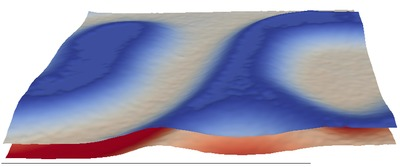
\includegraphics[height=4.5em]{cas3p2_fluo0p8_GDL4_2_t092_crop_resized.jpg}\\
	\SI{1}{\hour} 15 & 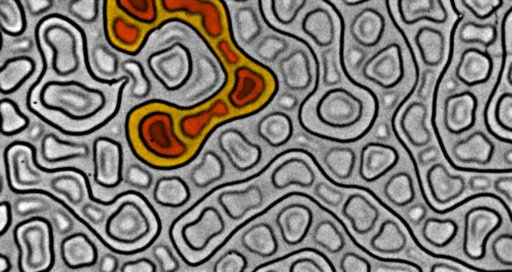
\includegraphics[height=4.5em]{prise_0360_color.jpg}&
	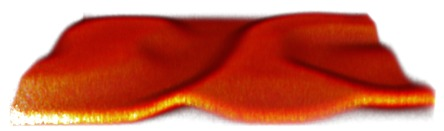
\includegraphics[height=4.5em]{cas3p2_fluo0p8_GDL4_2_t125_crop_resized.jpg}\\
	\SI{2}{\hour} 30 & 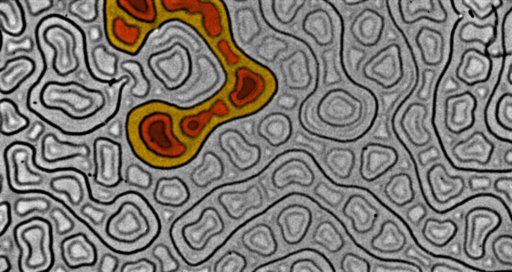
\includegraphics[height=4.5em]{prise_0799_color.jpg}&
	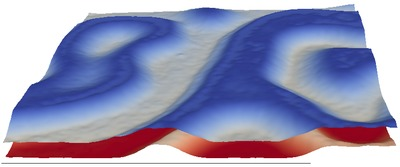
\includegraphics[height=4.5em]{cas3p2_fluo0p8_GDL4_2_t260_crop_resized.jpg}\\
};
\newdimen\mydima
\newdimen\mydimb
\pgfextractx{\mydima}{\pgfpointanchor{m-1-2}{east}}
\pgfextractx{\mydimb}{\pgfpointanchor{m-1-2}{west}}
 	\draw[line width=0.3em] (m-1-2.south west) ++(0.5em,0.5em)-- ++(0.17\mydima-0.17\mydimb,0);

\pgfextractx{\mydima}{\pgfpointanchor{m-1-3}{east}}
\pgfextractx{\mydimb}{\pgfpointanchor{m-1-3}{west}}
 	\draw[line width=0.3em] (m-1-3.south west) ++(1em,0) -- +(\mydima/1.272-\mydimb/1.272,0);
% 	\draw[ultra thick] ++(m-1-3.south west) -- ++(0.1\textwidth,0);

\begin{scope}[every node/.style={anchor=north east, text height=0.8em, text depth=0.2em}]
\node at (m-1-2.north west) {(a)};
\node at (m-1-3.north east) {(b)};
\end{scope}
%\draw (m.north west) rectangle +(\columnwidth, -\textheight);
\end{tikzpicture}

% 	\caption{Dynamics of pattern formation. Left: light transmission microscopy. Right: Reconstructed from fluorescent confocal microscopy. Scale bars are \SI{1}{\milli\metre}.}
%  	\label{fig:dynamics}
 %\end{figure}
	\caption{Dynamics of pattern formation. Left: light transmission microscopy. Right: Reconstructed from fluorescent confocal microscopy. Scale bars are \SI{1}{\milli\metre}.}
	\label{fig:dynamics}
\end{figure}

\begin{figure}
	\tikzsetnextfilename{acidification}
	\begin{figure}
\begin{tikzpicture}
	\begin{groupplot}[%
		group style={
			group name=g, group size=1 by 3,
			x descriptions at=edge bottom,
			vertical sep=0.5em,
			},
		xlabel={time (\si{\hour})},
		xmin=0,xmax=4, ymin=0,
		scale only axis,
		width=\columnwidth-4em,
		height=0.3\columnwidth,
		extra tick style={grid=major},%
		ylabel absolute, every axis y label/.append style={anchor=base, yshift=-1em}
		]
	\nextgroupplot[
		ymax=7, ylabel=pH,
		extra y ticks={4.6}, extra y tick labels={},%
		]
	\addplot+[no marks,black] table[x expr={\thisrowno{0}/3600.+0.05}]{Y189_28800s.pH};
	\node[base left=0] at (axis cs:8,4.6) {isoelectric};

	\nextgroupplot[
		ylabel={$G^\prime$ (\si{\pascal})}
		]
	\addplot+[no marks, black] table[x expr={\thisrowno{0}/3600.+0.05}]{Y235_28800s.prise};

	\nextgroupplot[
		ylabel={$\xi$ (\si{\micro\metre})}, restrict y to domain=0:10,
		]
	\addplot+[no marks, black] table[x expr={\thisrowno{0}/3600.+0.2}]{ech14_pore_size.txt};
	\addplot+[no marks, black] table[x expr={\thisrowno{0}/3600.+0.3}]{ech12_pore_size.txt};
	\end{groupplot}
\begin{scope}[every node/.style={anchor=south east, text height=0.8em, text depth=0.2em}]
\node at (g c1r1.south east) {(a)};
\node at (g c1r2.south east) {(b)};
\node at (g c1r3.south east) {(c)};
% \node[anchor=north east] at (g c2r1.north east) {(c)};
% \node[anchor=north east] at (g c2r2.north east) {(d)};
\end{scope}
	\end{tikzpicture}
\end{figure}
	\caption{Acid-induced protein gels properties behave non-monotonously with pH. (a) pH decrease in 4\%w sodium caseinate solution acidified by 4\%w GDL. Horizontal line indicates isoelectric pH of casen (b) Evolution of storage modulus measured in a rheometer (full adhesion to rotor and stator). (c) Evolution of pore size measured by confocal microscopy in a half coated microscopy cell (no adhesion to cell ceiling, syn\ae{}resis and swelling allowed).}
	\label{fig:acidification}
\end{figure}

\begin{figure}
	\tikzsetnextfilename{sideview}
	%\begin{figure}
\begin{tikzpicture}
\newdimen\mydima
\newdimen\mydimb
	\begin{groupplot}[%
		group style={
			group name=g, group size=1 by 2,
			x descriptions at=edge bottom,
			vertical sep=0.5em,
			},
		xmin=0, xmax=180, xtick={0,30,...,150},
		extra tick style={grid=major},%
		extra x tick labels={},%
		scale only axis,
		width=\columnwidth-4em,
		height=6\baselineskip,
		ylabel absolute, every axis y label/.append style={anchor=base, yshift=-1em, xshift=0.5em}
		]
	
	\nextgroupplot[ylabel={Volume (\%)}, ymin=20, ymax=100, ytick={40,60,80,100}]
	\addplot+[no marks,black] table[x expr={\thisrowno{0}+15}, y expr={\thisrowno{1}*100}]{relative_volume_excess_area_plis.txt}  coordinate[pos=0] (V0) (V0) |- (axis cs:0,100);
	\addplot+[only marks,Accent1, mark=+] table[x expr={\thisrowno{0}+15}, y expr={\thisrowno{1}*100}]{relative_volume_excess_area_plis_toi.txt};
	
	\nextgroupplot[ylabel={Excess area (\%)}, ymin=0, ymax=6, ytick={0,2,4,6}, 
	xlabel={time (min)}, every axis y label/.append style={xshift=-1em}]
	\addplot+[no marks,black] table[x expr={\thisrowno{0}+15}, y expr={\thisrowno{2}*100}]{relative_volume_excess_area_plis.txt};
	\addplot+[only marks,Accent1, mark=+] table[x expr={\thisrowno{0}+15},y expr={\thisrowno{2}*100}]{relative_volume_excess_area_plis_toi.txt};
	\end{groupplot}



\pgfmathsetlength{\mydima}{\columnwidth}
\begin{axis}[
	name=a,
	anchor=south east,
	at={($(g c1r1.above north east)+(0,\baselineskip)$)},
	width=\mydima, height=0.4\mydima, scale only axis,
	domain=-0.25*pi:2.25*pi, no markers, ymin=-2, ymax=3,xmin=0,xmax=2*pi,
	axis lines=none, xtick=\empty,
	]
	%tranche d'interet
	\fill[lightgray] (axis cs:0.425*pi,-2) rectangle (axis cs:0.575*pi,3);
	%gel et reperes
	\addplot+[Accent1, line width=0.1\mydima] {sin(deg(x))};
	\addplot+[draw=none,name path=top, yshift=0.055\mydima] {0.925*sin(deg(x))};
	\addplot+[draw=none,name path=bot, yshift=-0.055\mydima] {1.05*sin(deg(x))};
	\addplot+[name path=baseT, dashed, help lines,yshift=0.055\mydima]{0};
	\addplot+[name path=baseB, dashed, help lines, yshift=-0.055\mydima]{0};
	%epaisseur penchee
 	\path[name path=Z] (axis cs:pi-1,-100/pi^2) -- (axis cs:pi+1,100/pi^2);
	%chemin optique penche
 	\path[name path=D, name intersections={of=top and Z, by=Z2}] (Z2) -- +(0,-6\baselineskip);
	%epaisseur au max
	\path[name path=ZM] (axis cs:0.5*pi,-100/pi^2) -- (axis cs:0.5*pi,100/pi^2);
	%trace les chemins optiques
 	\draw[ultra thick, Accent2, name intersections={of=top and Z, by=Z2}, name intersections={of=bot and D, by=D1}, name intersections={of=top and ZM, by=ZM2}, name intersections={of=bot and ZM, by=ZM3}] (Z2) --(D1) (ZM2) -- (ZM3);
	%trace les épaisseurs h
	\draw[<->] (ZM2) -- (ZM3) node[midway, left] {$h$};
  	\draw[<->, name intersections={of=bot and Z, by=Z1}] (Z1) -- (Z2) node[midway, anchor=south east, inner sep=0] {$h$};
	%trace les autres épaisseurs
	\draw[<->] (axis cs:1.85*pi,0.75) -- (axis cs:1.85*pi,3) node[midway, right] {$H_2$}; 
	\draw[<->] (axis cs:1.85*pi,-0.75) -- (axis cs:1.85*pi,0.75) node[midway, right] {$h$};
	\draw[<->] (axis cs:1.85*pi,-0.75) -- (axis cs:1.85*pi,-2) node[midway, right] {$H_1$};
	\draw[->, name intersections={of=baseB and ZM, by=BW}] (BW) -- (ZM3) node[midway, left] {$A(t)$};
	\draw[<->] (axis cs:0,2.75) -- (axis cs:2*pi,2.75) node[midway, right,fill=white] {$\lambda$};
	
	%noms
	%\node[white] at (axis cs:1.5*pi,-1){gel};
	\node[Accent1] at (axis cs:1.5*pi,1.25){viscous ($\eta$)};
	\node[Accent1,above right] at (axis cs:0,-2){viscous ($\eta$)};
% 	\node[left,white, rotate=-20,inner sep=0.75em] at (axis cs:pi,0) {elastic ($B$)};
% 	\node[right,white, rotate=-20,inner sep=0.75em] at (axis cs:pi,0) {porous ($\alpha$)};
	\node[white, rotate=-20]  at (axis cs:pi,0) {elastic ($B$) \hspace{1.5em} porous ($\alpha$)};
	
	%pressures
	\node[above] at (axis cs:0.5*pi,1.75) {$P_2$};
	\node[below] at (axis cs:0.5*pi,-0.75) {$P_1$};
	\coordinate (Bm) at (axis cs:1.5*pi, -1.6);
	\node[single arrow, draw, anchor=tip, shape border rotate=270, inner xsep=0] at (axis cs:0.3*pi, 1.6) {$\sigma_\perp$};
	%flows
	\draw[->, lightgray, ultra thick] (axis cs:0.3*pi,1.4) -- (axis cs:0.3*pi, 0.3);
	\draw[->, lightgray, ultra thick] (axis cs:1.5*pi,-1.5) -- (axis cs:1.5*pi, -0.4) node[above] {Darcy flow};
	\draw[->, lightgray, ultra thick] (axis cs:1.45*pi,-1.8) -- (axis cs:0.6*pi, -1.8) node[pos=0.55, above] {Poiseuille flow};
	\draw[<-, lightgray, ultra thick] (axis cs:1.45*pi,1.8) -- (axis cs:0.6*pi, 1.8) node[pos=0.55, above] {Poiseuille flow};

	%axes
	\coordinate (Oo) at (axis cs:1.6*pi,1.75);
	\draw[->] (Oo) -- +(1.5em,0) node[right]{$x$};
	\draw[->] (Oo) -- +(0,1.5em) node[right]{$z$};
	
	%\node[below] at (axis cs:90,-1.75) (pb1) {$P_1$};
	%\node[above] at (axis cs:90,1.75) (ph2) {$P_2$};
	%\node[above] at (axis cs:270,1.75) (ph1) {$P_1$};
	%\node[below] at (axis cs:270,-1.75) (pb2) {$P_2$};
	%\draw[line width=0.1em, ->] (ph2) -- (axis cs:90,0.25) node[midway, left] {Darcy} node[midway, right] {$v$};
	%\draw[line width=0.1em, ->] (pb2) -- (pb1) node[midway, above] {Poiseuille} node[midway, below] {$u \sim \frac{\lambda}{H} v$};
\end{axis}
\fill[pattern=north east lines,pattern color=Accent2] (a.south west) rectangle +(\columnwidth,-\baselineskip) (a.north west) rectangle +(\columnwidth,\baselineskip);
\node[single arrow, draw, anchor=tip, shape border rotate=90, inner xsep=0] at (Bm) {$\sigma_\perp$};
%

	\matrix[matrix of nodes, matrix anchor=south east, inner sep=0, row sep=0.2em, nodes={anchor=west}, column sep=0.1em]  (m) at ($(a.north east) +(0,1.5\baselineskip)$) {
	\SI{10}{\minute} & 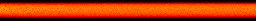
\includegraphics[width=0.88\columnwidth, height=0.054\columnwidth]{coupe_cloque_t000.png}\\
	\SI{23}{\minute} & 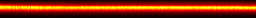
\includegraphics[width=0.88\columnwidth, height=0.052\columnwidth]{coupe_plis_t016.png}\\
	%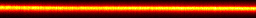
\includegraphics[width=\columnwidth, height=0.052\columnwidth]{coupe_plis_t032.png} & \SI{32}{\minute}\\
	\SI{35}{\minute} & 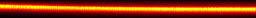
\includegraphics[width=0.88\columnwidth, height=0.046\columnwidth]{coupe_plis_t038.png} \\
	\SI{36}{\minute} & 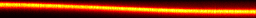
\includegraphics[width=0.88\columnwidth, height=0.046\columnwidth]{coupe_plis_t040.png} \\
	\SI{38}{\minute} & 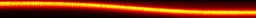
\includegraphics[width=0.88\columnwidth, height=0.046\columnwidth]{coupe_plis_t043.png} & \\
	\SI{44}{\minute} & 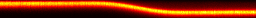
\includegraphics[width=0.88\columnwidth, height=0.046\columnwidth]{coupe_plis_t055.png}\\
	\SI{53}{\minute} & 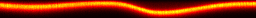
\includegraphics[width=0.88\columnwidth, height=0.046\columnwidth]{coupe_plis_t070.png} \\
	\SI{1}{\hour}~21 & 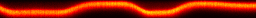
\includegraphics[width=0.88\columnwidth, height=0.046\columnwidth]{coupe_plis_t123.png} \\
	%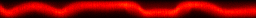
\includegraphics[width=\columnwidth, height=0.052\columnwidth]{coupe_plis_t332.png} & \SI{3}{\hour}~15\\
	};
\pgfextractx{\mydima}{\pgfpointanchor{m-1-2}{west}}
\pgfextractx{\mydimb}{\pgfpointanchor{m-1-2}{east}}
	\draw[line width=0.3em, white] ($(m-1-2.south west)+(0.75em,0.75em)$) -- +(0.0786\mydimb-0.0786\mydima,0);

%\draw (g c1r2.outer south east) rectangle +(-\columnwidth,\textheight);

\begin{scope}[every node/.style={anchor=north east, text height=0.8em, text depth=0.2em}]
\node[white] at (m-1-2.north east) {(a)};
\node[anchor=south east, inner ysep=1pt] at (a.north east) {(b)};
\node at (g c1r1.north east) {(c)};
\node at (g c1r2.north east) {(d)};
\end{scope}
\end{tikzpicture}
	
%\end{figure}
	\caption{Modelisation  and measurements. (a) Schematic side view of the cell. The constant thickness gel sheet (orange) is surrounded by water. Yellow lines show the path of transmitted light through the gel phase. A region of interest is highlighted in gray. (b) Confocal XZ cuts showing syn\ae{}resis, swelling and (cascade) wrinkling. Scale bar is \SI{100}{\micro\metre} (real size ratio). Evolution of (c) volume of the gel phase relative to cell volume and (d) excess area measured by confocal microscopy.}
	\label{fig:sideview}
\end{figure}

\begin{figure*}
	\tikzsetnextfilename{Darcy_vs_Poiseuille}
	\begin{figure}
\begin{tikzpicture}
\begin{groupplot}[group style={
			group name=g, 
	group size=3 by 1,
	horizontal sep=1em,
	y descriptions at=edge left,
			},
	scale only axis,
	width=0.333\textwidth-1.66em,
	xmin=0, xmax=3,ymin=0,ymax=3,
	ylabel={$\lambda$ measured (\si{\milli\metre})},
	cycle list name=black white,
	no marks]
\nextgroupplot[xlabel={$\lambda$ Darcy (\si{\milli\metre})},]
%\addplot+[only marks, error bars/.cd,x dir=both,y dir=both, x explicit,y explicit] table[x=D, x error=pmD, y=B, y error=pmB]{plis.txt};
\addplot+[only marks, error bars/.cd,x dir=both,y dir=both, x explicit,y explicit] table[x=D, x error=pmD, y=I, y error=pmI]{plis.txt};
\addplot+[black] {1*x};


\nextgroupplot[xlabel={$\lambda$ Poiseuille (\si{\milli\metre})},]
%\fill[gray] (axis cs:0.08,0.36) circle (5pt) (axis cs:0.36,0.46) circle (5pt);
%\addplot+[only marks, error bars/.cd,x dir=both,y dir=both, x explicit,y explicit] table[x=P, x error=pmP, y=B, y error=pmB]{plis.txt};
%\addplot+[forget plot] {3.5*x};
\addplot+[only marks, error bars/.cd,x dir=both,y dir=both, x explicit,y explicit] table[x=P, x error=pmP, y=I, y error=pmI]{plis.txt};
\addplot+[black] {1*x};
\addplot+[black, dashed] {0.81*x};
\addplot+[black, dotted] {0.56*x+0.28};
%\addplot+[only marks, error bars/.cd,x dir=both,y dir=both, x explicit,y explicit] coordinates{(0.41, 0.36) +-(0.05,0.04)};
%\node[anchor=north west, red, font=\footnotesize] (I) at (rel axis cs:0,1) {Inter blister};
%\node[anchor=north west, blue, font=\footnotesize] (B) at (I.south west) {Blister size};

\nextgroupplot[xlabel={$\lambda$ mixte (\si{\milli\metre})},]
%\fill[gray] (axis cs:0.08,0.36) circle (5pt) (axis cs:0.36,0.46) circle (5pt);
%\addplot+[only marks, error bars/.cd,x dir=both,y dir=both, x explicit,y explicit] table[x=P, x error=pmP, y=B, y error=pmB]{plis.txt};
%\addplot+[forget plot] {3.5*x};
\addplot+[only marks, error bars/.cd,x dir=both,y dir=both, x explicit,y explicit] table[x=M, x error=pmM, y=I, y error=pmI]{plis.txt};
\addplot+[black] {1*x};
\addplot+[black, dashed] {0.75*x};
\end{groupplot}
%\draw (g c1r1.outer north west) rectangle +(\textwidth, -\textheight);

\end{tikzpicture}
\end{figure}
	\caption{Comparing model predictions with measured wavelengths. Continuous line is the perfect match ($\lambda_{th}=\lambda_{xp}$), dashed line is the best linear fit through the origin (prefactor is 0.81 in a, 0.75 in b), dotted line is the best affine fit ($\lambda_{xp}=0.56\lambda_{th}+\SI{0.28}{\milli\metre}$).}
	\label{fig:DarcyPoiseuille}
\end{figure*}

\begin{figure}
	\tikzsetnextfilename{mesh}
	%\begin{figure}
\begin{tikzpicture}
\begin{groupplot}[group style={
			group name=g, group size=1 by 2,
			x descriptions at=edge bottom,
			vertical sep=0.5em,
			},
		scale only axis,
		width=0.5\columnwidth,
		xlabel={q (\si{\per\micro\metre})},
		ylabel={S(q) (a.u.)},
		domain=0.1:8,
		xmode=log,
		ymode=log,
		xmin=0.03, xmax=1e2,
		ymin=1e5, ymax=5e7,
		clip mode=individual,
	]
	\nextgroupplot
	\addplot+[only marks, mark options={scale=0.3, Accent1}] table{ech14_t008.Sq};
	\addplot+[black, no marks] {2.12455e+07/(1+(0.78346*x)^(2.39167)};
	\nextgroupplot%[ymin=6e5, ymax=1.5e7,]
	\addplot+[only marks, mark options={scale=0.3, Accent1}] table{ech6.Sq};
	\addplot+[black, no marks, domain=0.5:6.5] {4.92707951e+06/(1+(0.233*x)^(2.53)};
\end{groupplot}
\coordinate (topright) at  (g c1r1.outer north east -| g c1r2.outer south east);
\newdimen\mydima
\newdimen\mydimb
\pgfextracty{\mydima}{\pgfpointanchor{g c1r1}{north}}
\pgfextracty{\mydimb}{\pgfpointanchor{g c1r1}{south}}
\pgfmathsetlength{\mydima}{\mydima-\mydimb}
\node[inner sep=0, anchor=north west] at ($(topright|-g c1r1.north)+(-\columnwidth,0)$) (im1) {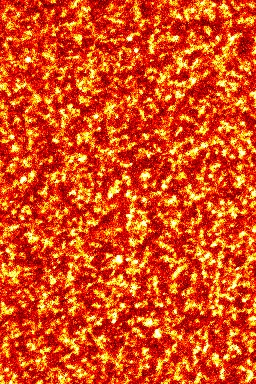
\includegraphics[height=\mydima]{ech14_t008.jpg}};
%scale bar 10 um
\draw[line width=0.3em] (im1.south west) ++(1em,1em) -- +(0.197\mydima,0);
\node[inner sep=0, anchor=north west] at ($(topright|-g c1r2.north)+(-\columnwidth,0)$) (im2) {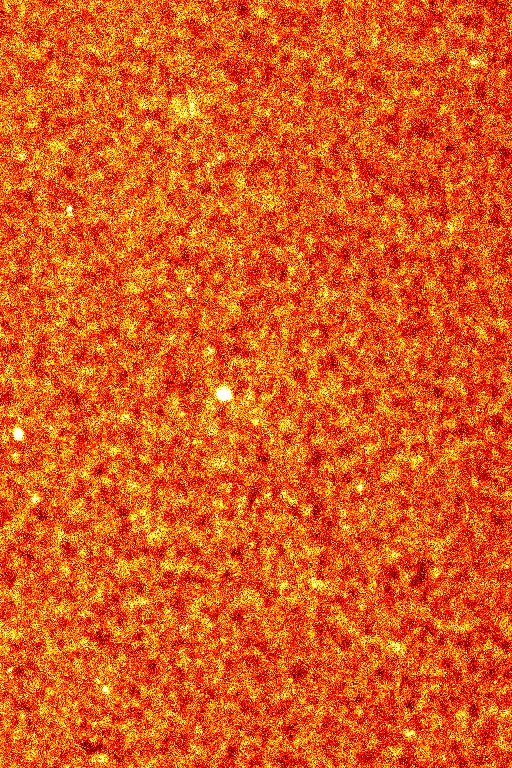
\includegraphics[height=\mydima]{ech6_x64_4.jpg}};
%scale bar 10 um
\draw[line width=0.3em] (im2.south west) ++(1em,1em) -- +(0.197\mydima,0);

\node[inner sep=0, above right= 0.1\mydima of g c1r1.south west] (sp1) {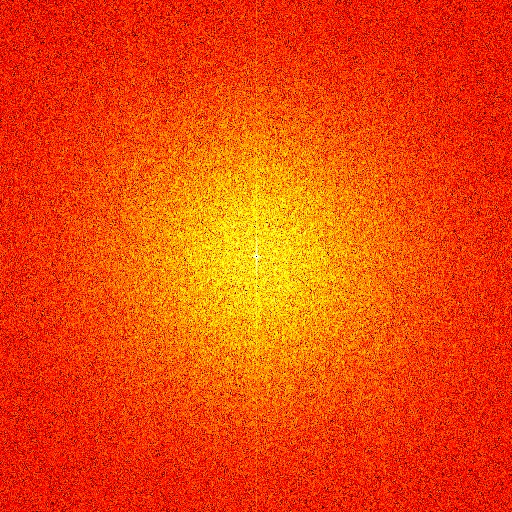
\includegraphics[width=0.5\mydima] {ech14_fft_t008.jpg}};
\draw[line width=0.3em] (sp1.south west) ++(1em,1em) --+(0.157\mydima,0); %10um-1
\node[inner sep=0, above right= 0.1\mydima of g c1r2.south west] (sp2) {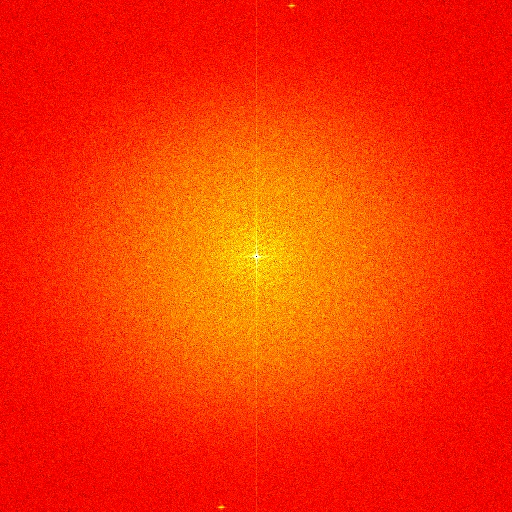
\includegraphics[width=0.5\mydima] {ech6_fft.jpg}};
\draw[line width=0.3em] (sp2.south west) ++(1em,1em) --+(0.157\mydima,0);%10um-1

\begin{scope}[every node/.style={anchor=north east, text height=0.8em, text depth=0.2em}]
\node[anchor=north west] at (im1.north east) {(a)};
\node at (g c1r1.north east) {(b)};
\node[anchor=north west] at (im2.north east) {(c)};
\node at (g c1r2.north east) {(d)};
\end{scope}

%\draw (topright) rectangle +(-\columnwidth,-\textheight);
\end{tikzpicture}
%\end{figure}
	\caption{Gel microstructure. (a) Detail of a confocal micrograph of a 4\%w casein, 4\%w GDL in water, when only the slide is coated (not the cover slip). Time corresponds to the minimum in mesh size. Scale bar is \SI{10}{\micro\metre}. (b) Corresponding radial averaged Fourier transform. Black line is the best fit by Eq.XXX with $\xi=\SI{2.0}{\micro\metre}$ and $d_{3D}=2.27$. Inset shows the center of the non radial average spectrum (arbitrary logarithmic color scale). Scale bar is \SI{10}{\per\micro\metre}. (c-d) Idem in a 50\%w glycerol solvent, with $\xi=\SI{0.3}{\micro\metre}$ and $d_{3D}=3$.}
	\label{fig:mesh}
\end{figure}

\begin{figure*}
	\tikzsetnextfilename{permeability}
	% \begin{figure*}
\begin{tikzpicture}
\begin{groupplot}[
	group style={
			group name=g, group size=2 by 1,
			y descriptions at=edge left,
			horizontal sep=1em,
			},
	width=0.4\textwidth,
	height=0.5\columnwidth,
	xlabel={$t$ (hours)},
	ylabel={$z-z_\infty$ (\si{\centi\metre})},
	xmin=0, ymax=0, ymin=-5,
	clip mode=individual,
	]
	\nextgroupplot[xmax=3]
	\addplot+[only marks, mark options={scale=0.5, Accent2}] table[x expr={\thisrowno{0}/3600}, y expr={-\thisrowno{1}*100}]{montee_cas4_GDL4.txt};
	\addplot+[no marks, black, domain=0:3] {-5*exp(-x/56.6*60)};
	%H=2.3mm
	\nextgroupplot[xmax=10,xlabel={$t$ (days)},]
	\addplot+[only marks, mark options={scale=0.5, Accent1}] table[x expr={\thisrowno{0}/3600/24}, y expr={-\thisrowno{1}*100}]{montee_cas4_GDL4_gly50.txt};
	\addplot+[no marks, black, domain=0:10] {-3.5*exp(-x/100*24)};
	%H=4mm
	
\end{groupplot}


\node[minimum height=0.25\columnwidth, minimum width=0.5\columnwidth, fill=gray!50, anchor=south west] (whey) at ($(g c2r1.outer south east)+(-\textwidth,0)$) {};
\begin{scope}[every node/.style={minimum width=0.05\columnwidth}]
%where the tubes will be
\node[minimum height=0.4\columnwidth, anchor=west] (tubel) at ($(whey.north)+(-0.1\columnwidth,0)$) {};
\node[minimum height=0.4\columnwidth, anchor=east] (tuber) at ($(whey.north)+(0.1\columnwidth,0)$) {};
%Jurin in tubel
\node[minimum height=6em, anchor=west, fill=gray!50] (wheyinfty) at (tuber.west)  {};
%lack of liquid at t2
\node[minimum height=2em, anchor=north east, fill=white] (wheyt2) at (tubel.east) {};
%lack of liquid at t1
\node[minimum height=\baselineskip, anchor=north] (wheyt1) at (wheyt2.south) {};
\end{scope}
%gel
\fill[Accent1] (wheyt1.south west) +(0,-0.5em) rectangle (tubel.south east);
%draw tubes
\draw[very thick] (tubel.south west) -- (tubel.north west) (tubel.south east) -- (tubel.north east)
(tuber.south west) -- (tuber.north west) (tuber.south east) -- (tuber.north east);

%labels
\draw[<-] (wheyinfty.north east) -- +(1em,0) node[right]{$z_\infty$};
\draw[<-] (wheyt2.south west) -- +(-1em,0) node[left]{$z(t)$};
%\draw[<-] (wheyt1.south east) -- +(1em,0) node[right]{$z(t_1)$};
\draw  (wheyt1.south west) ++(0,-0.5em) -- +(-1em,0) coordinate[pos=0.9] (Ht) (tubel.south west) -- +(-1em,0) coordinate[pos=0.9] (Hb);
\draw[<->] (Ht) -- (Hb) node[midway, left] (H) {$H$};
\draw[<-] (H -| tubel) -- +(0.05\columnwidth,0) node[right]{gel};
\node[anchor=north east] at (whey.north east) {buffer};
\node[anchor=north] at (tubel.north) (l1){$1$};
\node[anchor=north] at (tuber.north) {$2$};
%\draw[->] (whey.south west) ++(45:0.075\columnwidth) -- +(0,0.1\columnwidth) node[above] {$x$};
%\draw (l1.north-|whey.west) rectangle +(\textwidth,-\textheight);

\begin{scope}[every node/.style={anchor=north west, text height=0.8em, text depth=0.2em}]
\node at (l1.north-|whey.west) {(a)};
\node at (g c1r1.north west) {(b)};
\node at (g c2r1.north west) {(c)};
\end{scope}


\end{tikzpicture}
% \caption{Schematic representation of permeability measurement.}
% \label{fig:tubexp}
% \end{figure*}
	\caption{Permeability measurements. (a) Schematic representation of the experiment. (b-c) Evolution of the height of the interface in tube 1 relative to the final height in tube 2. Black line is the best exponential fit $Ae^{-t/\tau}$. (b) Gel is 4\%w casein, 4\%w GDL in water, $H=\SI{2.3}{\milli\metre}$ and $\tau=\SI{57}{\minute}$. (c) Idem in 50\%w glycerol, $H=\SI{4}{\milli\metre}$ and $\tau=\SI{100}{\hour}$.}
	\label{fig:permeability}
\end{figure*}

\begin{figure}
	\tikzsetnextfilename{growth}
	\begin{figure}
\begin{tikzpicture}
\begin{groupplot}[
	group style={
			group name=g, group size=1 by 2,
			%y descriptions at=edge left,
			vertical sep=4em,
			},
	width=\columnwidth,
	ylabel absolute, every axis y label/.append style={anchor=base, yshift=-0.3em},
	]
	\nextgroupplot[
		xlabel={time (\si{\minute})},
	ylabel={$A(t)$ (\si{\micro\metre})},
	ymode=log, ymin=5,
	restrict x to domain=17:30,
	ytick={5,10, 20, 50}, yticklabels={5,10,20,50},
	clip mode=individual,
	]
	\addplot+[Accent1, only marks,mark=+] table[x expr={\thisrowno{0}/60.+3}]{cas3p2_fluo0p8_GDL4.ampl};
	%\addplot[black, no marks, domain=22:25] {exp((x-100)/120.*60)};
	\addplot[black, no marks, domain=23:25] {exp((x-19.75)/1.3)};
	
	
	\nextgroupplot[
	xmin=0, xmax=1000, xtick={0,250, 500, 750}, xlabel={$x$ (\si{\micro\metre})},
	ymin=0, ymax=50, ylabel={$z_\text{bottom}(x,t)$ (\si{\micro\metre})},
	cycle list={
		{Accent2}, 
		{black!15!Accent2},
		{black!30!Accent2},
		{black!45!Accent2},
		{black!60!Accent2},
		{black!75!Accent2},
		{black, thick}
	},
	no marks,
	]
	\foreach \x in {2,3,..., 8}
		\addplot table[y index=\x]{alts_bottom_cloque.txt};
		
	\draw[ultra thick, Accent1] (axis cs:580,0) -- (axis cs:580,50);
	
\end{groupplot}

\begin{scope}[every node/.style={anchor=north west, text height=0.8em, text depth=0.2em}]
\node at (g c1r1.north west) {(a)};
\node at (g c1r2.north west) {(b)};
\end{scope}
%\draw (g c1r1.outer north west) rectangle +(\columnwidth,-\textheight);
\end{tikzpicture}
\end{figure}
	\caption{Growth of the instability. (a) Evolution of the gel velocity $v$, integrated over the whole surface. Inset: Evolution of the amplitude (peak to peak measurement) in semi logarithmic scale. Black line is the best exponential fit with $\tau=\SI{90}{\second}$. (b) Evolution of the bottom profile of the gel from the onset of instability (yellow) to the contact to both walls (brown). Note that the lateral size of the blister evolve in this regime. Thick black curve is the profile at much longer time. Note that blister foot (highlighted by the orange vertical line) has not moved since contact.}
	\label{fig:growth}
\end{figure}

\end{document}